\subsection{Reconocimiento de caracteres como un problema de clasificación de imágenes naturales}
\label{subsection: wang_recon_caracteres}
	
	El reconocimiento de caracteres es la primera etapa en el pipeline de procesamiento que desarrollaron Wang et al. Dada una imagen, inicialmente es necesario detectar las potenciales ubicaciones de los caracteres dentro de la misma. Para lograr esto, los autores realizan una detección a múltiple escala usando un algoritmo de clasificación de ventana deslizante. Esta ventana al comienzo tiene un tamaño fijo, y  recorre la imagen detectando potenciales caracteres contenidos en ella. Luego aumenta su tamaño con el objetivo de poder detectar caracteres más grandes. Supongamos que la ventana está ubicada en una zona de la imagen donde hay un carácter a detectar. Si quisieramos reconocer ese carácter, sería necesario compararlo con los 62 posibles caracteres existentes. Dado que hay muchos símbolos involucrados, los autores tienen que lograr clasificar cada nueva entrada dentro de las 62 posibles clases. Estas clases estan formadas por los caracteres alfabéticos, en minúscula y mayúscula, 52 en total, y numéricos, 10 en total). Dada la gran cantidad de clases, y que los sistemas que emplean esquemas de reconocimiento de caracteres usualmente deben funcionar en tiempo real y evaluar una gran cantidad de ventanas, se tiene asociado un gran costo computacional. El clasificador \textit{Random Ferns} (ver \ref{subsection:ferns}), ha demostrado ser una buena opción por su eficiencia y capacidad de manejar múltiples clases.
	
	%Para entrenar a este clasificador, los autores realizan dos pruebas diferentes. La primera consta de entrenar al clasificador con imágenes recortadas de caracteres que obtuvieron del dataset público \textit{Chars74k-15} (ver sección X). La segunda prueba la realizan sobre datos sintéticos creados por ellos mismos. Dada la gran variabilidad de apariencias que hay en las imágenes reales y a lo difícil que es recolectar un conjunto de este tipo, es que surge esta segunda prueba. Esto supone una gran ventaja por la cantidad ilimitada de datos que se puede manejar. Este enfoque fue aprovechado por los autores, que sintetizaron alrededor de 1000 imágenes por carácter usando 40 fuentes. El objetivo de esto era obtener imágenes de caracteres que se asemejaran a las imágenes reales. Para lograr esto, a cada imagen de fuente le aplicaban una serie de transformaciones que alteraban su aspecto en un intento de imitar los diferentes aspectos que podía tener una imagen natural. Como se puede observar en la Figura \ref{fig: Datos sinteticos Wang}, estas imágenes tienen variaciones en el color de la letra y el fondo, como así también la inclinación del carácter y su posición dentro de la imagen.
	
		\begin{figure}[htbp]
			\centering
			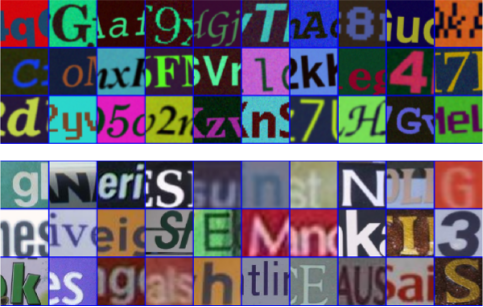
\includegraphics[scale=0.5]{img/synth_data_wang.png}
			\caption[Datos sintéticos Wang]{Arriba se puede ver el conjunto de imágenes sintéticas creadas por Wang et. al. Estas imágenes tienen una dimensión de 48x48 píxeles e intentan imitar a las imágenes reales. Abajo se puede observar un conjunto de imágenes reales recortadas que  fueron extraidas del dataset ICDAR. Fuente: Wang et. al. \cite{wang}.}
			\label{fig: Datos sinteticos Wang}
		\end{figure}
	
	Para poder reconocer un símbolo, se tienen que extraer aquellas características que lo distingue de otros símbolos (sección \ref{subsection:feature}), es decir, aquello que lo hace único. Una forma de lograr esto es a través de los gradientes de la imagen (ver apéndice \ref{section:Apendice-C}). En la literatura de clasificación y reconocimiento en imágenes naturales, un vector de características muy empleado es HOG (\textit{Histogram of Oriented Gradients}). Es un descriptor en $\mathbb{R}^N$ que modela la distribución del gradiente de una imagen. HOG ha demostrado ser una representación robusta de las imágenes en el problema relacionado a la clasificación de imágenes naturales \cite{DT05}. 
	
	Para el entrenamiento de \textit{Random Ferns}, se tienen los descriptores HOG de cada imagen para cada una de las 62 clases. Sin embargo, no es suficiente para poder empezar a entrenar ya que \textit{Random Ferns} requiere del uso de descriptores binarios. Es por eso que, siguiendo la propuesta de Wang et. al., se propone binarizar los descriptores HOG en lugar de generar descriptores binarios directamente a partir de imágenes.
	
	%para la clasificación pues son fáciles de computar, almacenar y escala con la cantidad de clases. En su trabajo, especifican que los vectores binarios consisten en la aplicación de umbrales elegidos aleatoriamente sobre entradas elegidas al azar del vector HOG. Un vez binarizados los descriptores es posible entrenar al clasificador y dejarlo listo para clasificar nuevas instancias de imágenes de caracteres.
	
	El pipeline de reconocimiento finaliza una vez que se ha detectado un carácter, con una técnica denominada \textit{supresión de los máximos} (\textit{NMS} por sus siglas en inglés). Esta técnica se aplica sobre el carácter detectado y es una técnica muy usada en los algoritmos de visión por computadora. Básicamente, suprime los píxeles en la imagen que no son máximos locales, con respecto a los píxeles vecinos, a lo largo de la dirección del gradiente.

\subsubsection{Histograma de Gradientes Orientados}
\label{subsubsection:hog}

	Los Histogramas de Gradientes Orientados o HOG, por sus siglas en inglés, son descriptores de características utilizados en visión por computadora y en el procesamiento de imágenes con el objetivo de realizar detección de objetos. Fueron introducidos por N. Dalal y B. Triggs en~\cite{DT05} con el propósito de realizar detección de personas. Sin embargo, su uso no se limita solamente a esa área, sino que pueden ser utilizados en otras áreas como la detección de caracteres tal como hicieron Wang et al. en \cite{wang}.
	
	Todas las imágenes, como por ejemplo la presentada en la Figura~\ref{fig: Vector HOG}\textit{A}, contienen estructuras locales cuyas apariencias y formas pueden ser descriptas por la distribución de los gradientes de intensidad, como se puede observar en la Figura~\ref{fig: Vector HOG}\textit{B}.
	Un descriptor HOG es un vector compuesto por una combinación de histogramas que representan los gradientes de intensidad en distintas regiones de una imagen. Estos descriptores se obtienen dividiendo a la imagen en regiones de tamaño fijo llamadas celdas, como se puede observar en la Figura~\ref{fig: Vector HOG}\textit{B}, y posteriormente, por cada celda, calculando un histograma de gradientes para los píxeles en esa celda, Figura ~\ref{fig: Vector HOG}\textit{C}.
	Luego, se agrupan las celdas en bloques, Figura \ref{fig: Vector HOG}\textit{C}, y se normaliza cada uno utilizando la norma $L_{2}$. Esto se hace con el objetivo de obtener un descriptor robusto ante los cambios en la iluminación, entre otros. Por ejemplo, consideremos la Figura \ref{fig: Vector HOG}\textit{C}. Sea $b_{nm}~n,m=1,\dots,3$, un bloque $2 \times 2$ tal que 
	
	$$b_{nm} = (h_{nm}, h_{n(m+1)}, h_{(n+1)m}, h_{(n+1)(m+1)})$$
	
	donde $h_{ij}$ representa la celda ubicada en la fila $i$ columna $j$. Como se puede observar, en la figura aparece un área resaltada que hace referencia al bloque $b_{11}$. La norma $L_{2}$ para $b_{11} = (h_{11}, h_{12}, h_{21}, h_{22})$ se obtiene de la siguiente manera:
	
	 $$||b_{11}||_2 = \sqrt{h_{11}^{2} + h_{12}^{2} + h_{21}^{2} + h_{22}^{2}}$$
	 luego se normaliza el bloque $b_{11}$ 
     $$b_{11}' = \frac{b_{11}}{||b_{11}||_2} $$
     
	 Finalmente, el descriptor HOG se obtiene de concatenar los histogramas obtenidos como muestra la Figura~\ref{fig: Vector HOG}\textit{D}.
	
	%El descriptor HOG mantiene una cuantas ventajas con respecto a otros métodos descriptores. Dado que el descriptor HOG opera en celdas localizadas, el método mantiene la invarianza a transformaciones geométricas y fotométricas, excepto para la orientación de objetos. Dichos cambios sólo aparecerían en regiones espaciales grandes~\cite{DT05}.
	
		\begin{figure}[htbp]
			\centering
			\centerline{ 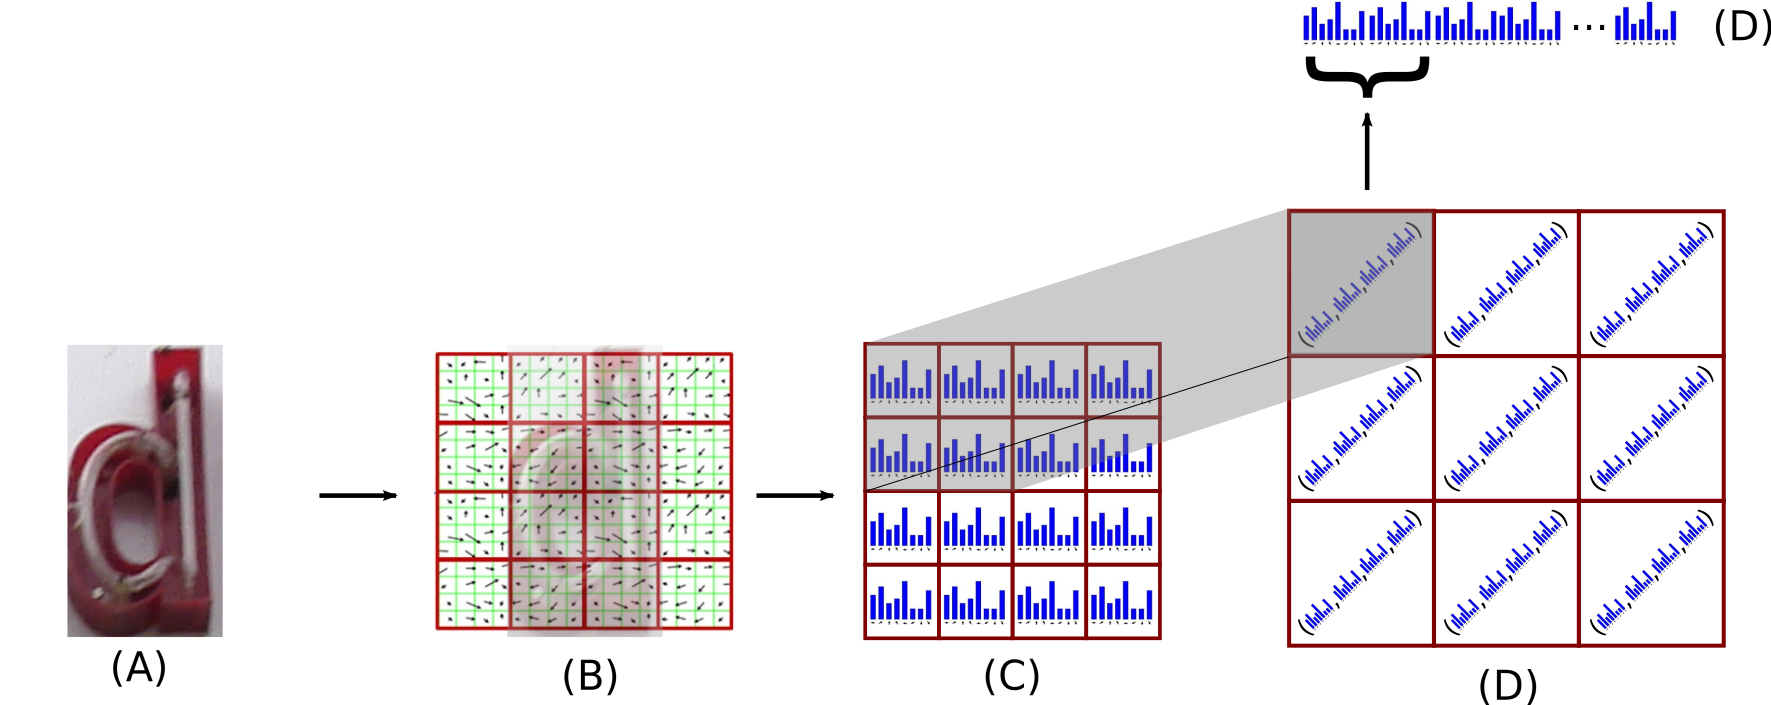
\includegraphics[scale=0.27]{img/hog/hog.png} }
			\caption[Extracción HOG]{Formación del vector de características HOG}
			\label{fig: Vector HOG}
		\end{figure}
		
	En el área de visión por computadora, los descriptores HOG son considerados estado del arte. Los mismos han demostrado ser útiles en la clasificación de imágenes como se puede apreciar en el trabajo de Wang et al.~\cite{wang} a donde se ha entrenado el clasificador Random Ferns con estos. Incluso la performance obtenida con estos descriptores en dicho trabajo supera a la mayoría de los descriptores evaluados en el trabajo de De Campos et al.~\cite{dCBV09} bajo las mismas condiciones de entrenamiento.
	
\subsubsection{Binarización}
\label{subsubsection:binarizacion}

	Una de las condiciones para poder usar los descriptores HOG en el clasificador \textit{Random Ferns}, es que los mismos tienen que estar binarizados. Los descriptores binarios son fáciles de computar, son compactos, se pueden almacenar fácilmente y son fáciles de comparar. En cambio, los descriptores originales tienen alta dimensionalidad y requieren sistemas con más memoria, capacidad de almacenamiento y procesamiento. Muchos sistemas en tiempo real como el reconocimiento de objetos, \cite{SJC08}, y en el agrupamiento de puntos clave, \cite{OFL07}, han incorporado este enfoque por su utilidad.
	
	 Para binarizar los descriptores HOG se requiere de un vector umbral. El mismo, una vez  calculado, se encarga de binarizar todos los descriptores tanto del conjunto de entrenamiento como del conjunto de evaluación. Dicho umbral se calcula utilizando solamente el conjunto de entrenamiento y se obtiene de la siguiente manera:
		
		\begin{itemize}
		
			\item Dado $N$ descriptores HOG de dimensión $D$, se forma una matriz $Q \in \mathbb{R}^{N \times D}$ donde cada fila representa un vector.
			\item Por cada uno de los $N$ vectores originales $v=(v_1,\dots,v_D)$, se seleccionan $X$ dimensiones al azar de $v$, con reemplazo, obteniendo de esta manera un vector $z = (z_1,\dots,z_X) \textit{, con } z_i=x_{\hat{i}},~\hat{i} \in \{1,\dots,D\}$, donde $\hat{i}$ es un número al azar en el rango $\{1,\dots,D\}$.
			\item Posteriormente, se procede a binarizar $z$ de la siguiente manera. Dado una dimensión $z_i$ de $z$, se aplica una función de umbralización sobre la \textit{i-esima} columna de $Q$, la función puede ser el calculo de la mediana, la media, bootstrap, entre otros. Se obtiene de esta manera $w_i \in \mathbb{R}$. Luego, si $z_i \geq w_i$ se le asigna $1$ a esa dimensión y $0$ en caso contrario. El vector umbral $W$ surge de aplicar $X$ veces la función de umbralización sobre la matriz $Q$, recordar que hay dimensiones repetidas en $z$.
						
		\end{itemize}
	
	A la binarización se la puede expresar con la siguiente composición de funciones:
	
	$$h \circ g:\mathbb{R}^{D} \rightarrow \{ 0, 1\}^{X}$$
	
	donde
	
	$$\textit{h: }\mathbb{R}^{X} \rightarrow \{ 0, 1\}^{X}$$
	
	$$\textit{g: }\mathbb{R}^{D} \rightarrow \mathbb{R}^{X}$$
	
	
	$\textit{g: }\mathbb{R}^{D} \rightarrow \mathbb{R}^{X}$ es una función definida de la siguiente manera. Dado un vector  $x=(x_1, \dots, x_D)$:

	\begin{equation}
	\label{eq: g_equation}
		g(x) = z = (z_1,\dots,z_X) \textit{, con } z_i=x_{\hat{i}},~\hat{i} \in \{1,\dots,D\}
	\end{equation}		
	
	En \ref{eq: g_equation} $\hat{i}$ representa un entero elegido de manera aleatoria en el rango $\{1,\dots,D\}$. Luego, una vez obtenido $z$, aplicamos la función $h$
	\begin{equation}
	\label{eq: h_equation}
		(y_1,\dots,y_X) = h(z) = (h_1(z_1),\dots,h_X(z_X))
	\end{equation}
	donde
	\[
    		h_{i}(z_i) = 
		\begin{cases}
    			1 & \text{si } z_i \geq w_{i}\\
    			0 & \text{caso contrario}
		\end{cases}
	\]

	$w_{i} \in \mathbb{R}$ representa al valor obtenido de haber aplicado una función de binarización a la columna \textit{i-esima} de la matriz  $Q$. Las funciones de binarización que se utilizan en este trabajo y que forman los vectores umbrales son: \textit{media}, \textit{mediana}, \textit{exponencial} y \textit{bootstrap}. A continuación se procede a explicar en detalle cada función.
	
	Dada la columna ``\textit{i-esima}'' de la matriz $Q$ representada por $C_i = (c_{i_1}, \dots, c_{i_j})$, con $j=1, \dots, N$ luego:

	\begin{itemize}
	
	\item \textbf{Media:}
	
	La \textbf{media} es una función $\textit{b: }\mathbb{R}^{N} \rightarrow \mathbb{R}$ tal que:
	
	$$b(C_i) = \frac{\sum_{j=1}^N c_{i_j}}{N} $$

	\item \textbf{Mediana:}
	
	La \textbf{mediana} es una función $\textit{b: }\mathbb{R}^{N} \rightarrow \mathbb{R}$ cuyo único requisito es que el vector esté ordenado. Sea \textit{dim(C)} la dimensión del vector $C$, luego:
	
	\[
    		b(C_i) = 
		\begin{cases}
    			\frac{c_{i_{\frac{dim(C)}{2}}} + c_{i_{\frac{dim(C)}{2}+1}}}{2} & \text{si dim(C) es par}\\
    			\frac{c_{i_{\frac{dim(C)}{2}}}}{2} & \text{caso contrario}
		\end{cases}
	\]
	
	\item \textbf{Bootstrap}
	
	Al igual que la \textit{media} y la \textit{mediana}, \textbf{bootstrap} es una función $\textit{b: }\mathbb{R}^{N} \rightarrow \mathbb{R}$ tal que, dado $c_{i_k} \in C_{i}$ una dimensión aleatoria de $C_{i}$ luego:
	
	$$ b(C_i) = c_{i_k} $$

	\item \textbf{Exponencial}
	
	La elección de la distribución exponencial se basa en las observaciones de que las dimensiones, de manera individual, se las puede aproximar con una distribución exponencial, ver Figura \ref{fig: exponential-fit}. Para una dimensión en particular, el parámetro lambda fue estimado en base a un criterio de máxima verosimilitud a partir de las muestras para esa dimensión.
	
	$$\hat{\lambda} = \frac{\sum_{j=1}^N c_{i_j}}{N} $$
	
		\begin{figure}[htbp]
			\centering
			\centerline{ 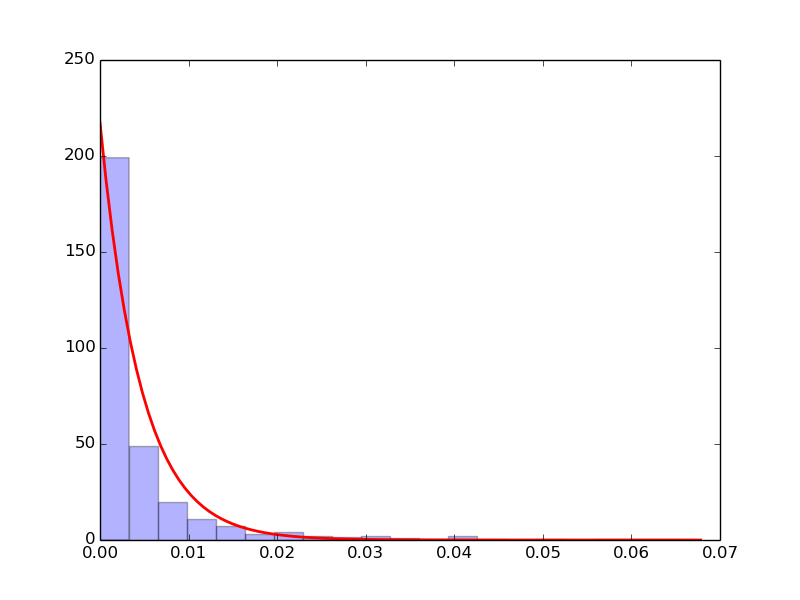
\includegraphics[scale=0.50]{img/histograma-curva.png} }
			\caption[Histograma con curva exponencial]{Histograma obtenido para una dimensión individual y la aproximación de esta a una distribución exponencial a través de la curva en rojo.}
			\label{fig: exponential-fit}
		\end{figure}
		
	
	\end{itemize}